\section{Extreme-token Phenomena in the Bigram-Backcopy Task}\label{sec:bb_task}


In this section, we analyze simple transformers trained on the Bigram-Backcopy (BB) task, a simple model that exhibits extreme-token phenomena. We demonstrate the \textit{active-dormant mechanism} (cf.\ Claim~\ref{claim:active-dormant}) and \textit{mutual reinforcement mechanism} (cf.\ Claim~\ref{claim:mutual-reinforcement}) within the BB task and provide predictions for the behavior of sink tokens, which will be validated through LLM experiments in the following section. 

The Bigram-Backcopy task is a data-generation model that consists of two sub-tasks: \textit{Bigram-transition} and \textit{Backcopy}. In this model, each sequence begins with the \bos~token, followed by tokens sampled according to a pre-determined bigram transition probability $\transit$ (in other words, a Markov chain). When specific trigger tokens are encountered, instead of sampling according to the transition $\transit$, the preceding token is copied to the next position. An illustration of the Bigram-Backcopy task is provided in \Cref{fig:bbm-dgp}. Following \citet{bietti2024birth}, we select the transition $\transit$ and the vocabulary $\vocab$ with $| \vocab | = V = 64$ based on the estimated character-level bigram distribution from the \textit{tiny Shakespeare} dataset. In all experiments, the set of trigger tokens, $\cT$, is fixed and consists of the $\abs{\cT}=3$ most frequent tokens from the unigram distribution. Consequently, the non-trigger token set, $\vocab\setminus \cT$, comprises $61$ tokens.

\subsection{One-layer transformer exhibits \attnsink s and \valuedrain s}

On the \bb~task, we pre-train a standard one-layer transformer with a single SoftMax \attn~head and one \mlp~layer. Unless otherwise specified, the model is trained using Adam for $10,000$ steps, achieving near-optimal prediction accuracy. Detailed training procedures are provided in Appendix~\ref{appsec:experiment-detail}. Figure~\ref{fig:bbm-attn} shows that the trained transformer exhibits the \attnsink~phenomenon, where the \bos~token captures a significant proportion of the attention weights. More importantly, the attention weights display interpretable patterns: all non-trigger tokens exhibit \attnsink s, while the attention for trigger tokens is concentrated on their preceding positions. Additionally, Figure~\ref{fig:bbm-value} reveals a value-state drain phenomenon similar to that observed in LLMs, suggesting that, for non-trigger tokens, the \attn~head contributes minimal value to the residual stream. We provide additional attention patterns on different input sequences in \Cref{appsec:additional-attn-maps}.

\begin{figure}[t]
  \centering
  \begin{minipage}{0.38\textwidth}
      \centering
      \subcaption{\small The Bigram-Backcopy task}
      \label{fig:bbm-dgp}
      \vspace{-.2em}
      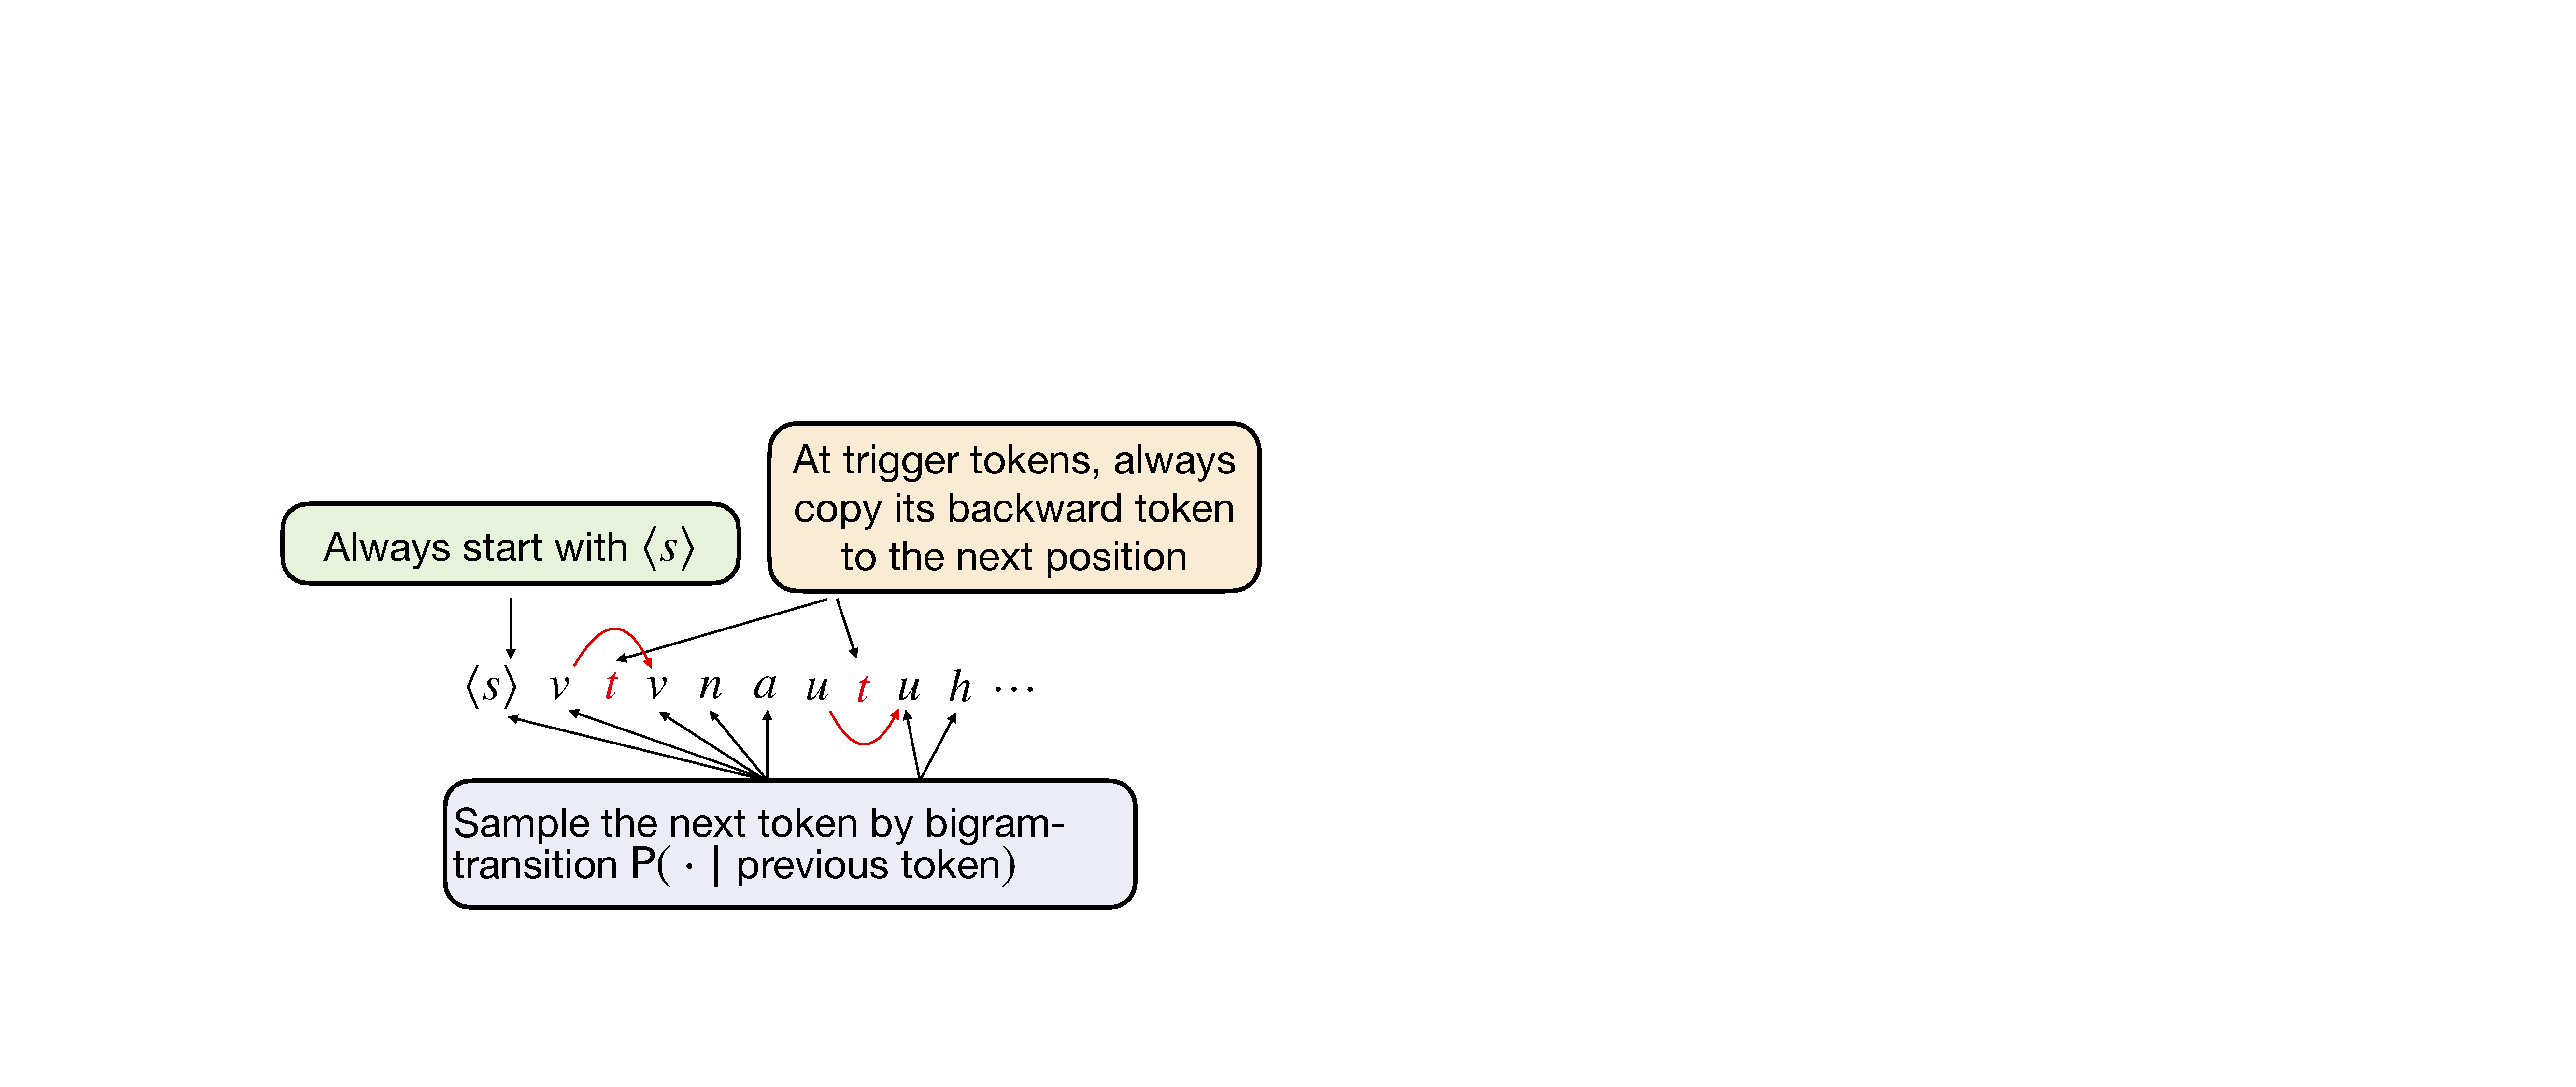
\includegraphics[width=\linewidth]{Figures/BBM/BBM.pdf}
  \end{minipage}
  % \hspace{-1em}
  \begin{minipage}{0.26\textwidth}
      \centering
      \subcaption{\small Attention pattern}
      \label{fig:bbm-attn}
      \vspace{-.2em}
      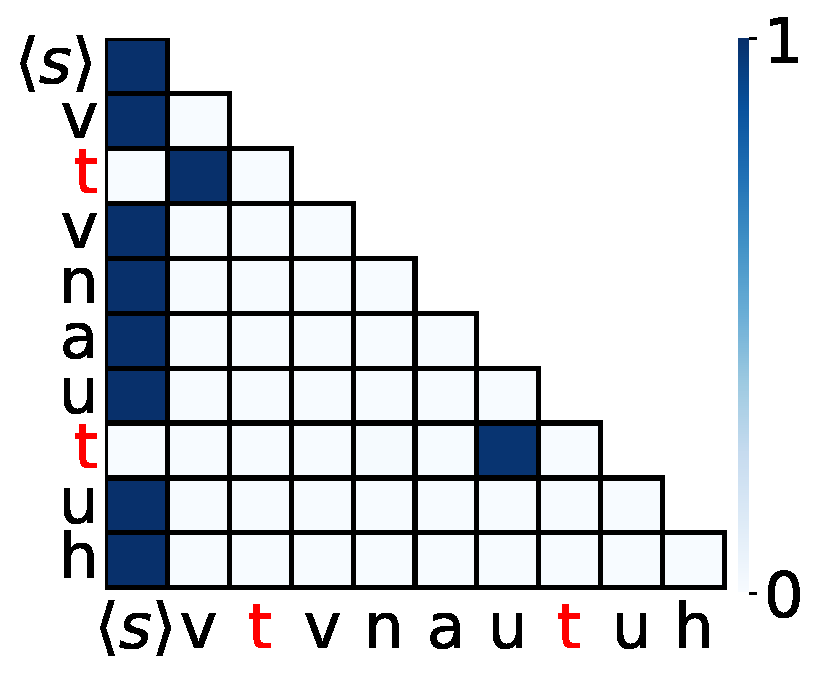
\includegraphics[width=\linewidth]{Figures/BBM/attn_fig1.pdf}
  \end{minipage}
  % \hspace{-1em}
  \begin{minipage}{0.27\textwidth}
      \centering
      \subcaption{\small Small value states}
      \vspace{0pt}
      \label{fig:bbm-value}
      \vspace{-.2em}
      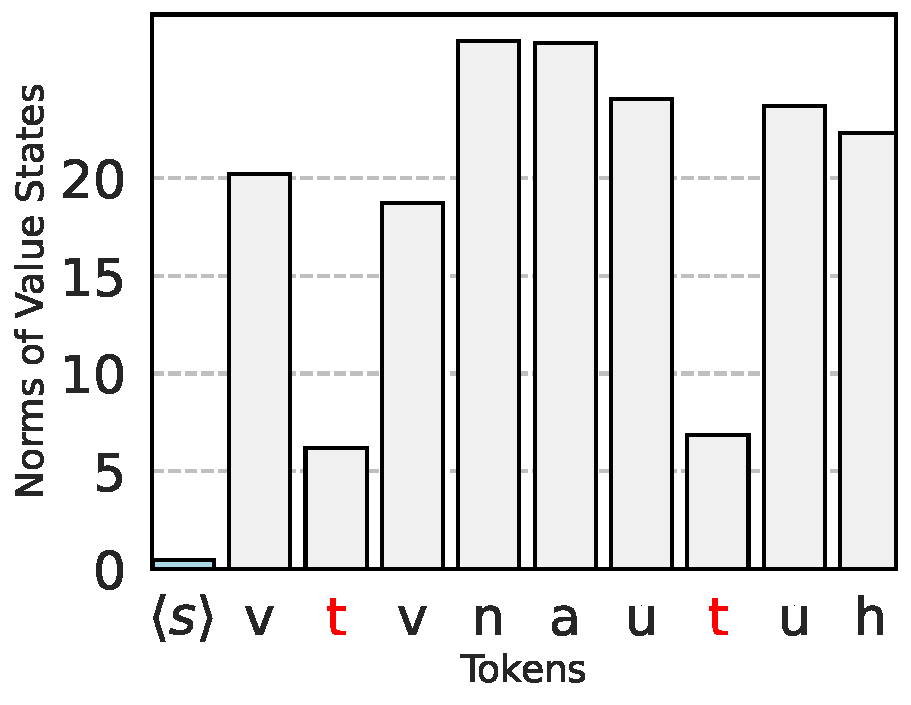
\includegraphics[width=\linewidth]{Figures/BBM/value_states_white.pdf}
  \end{minipage}
  % \vspace{-1em}
  \caption{\small \textbf{Experiments on the Bigram-Backcopy task.} 
  %\sm{Consistently use left (a) instead of reference to self} 
  \textit{Left (a)}: The data generation procedure for the Bigram-Backcopy task. Here we fix `t', `e', and the space character (` ') as trigger tokens. The BB task samples bigram transitions for non-trigger tokens and backcopies for trigger tokens.  \textit{Middle (b)}: The attention map of a given prompt. Trigger tokens are marked in red. The attention head at non-trigger tokens is dormant and displays attention sinks.  \textit{Right (c)}: The value state norms for the prompt. The \bos~token has the smallest norm. 
  % \sm{Figure (a): $\sf P$. Figure (b): Add grid. Figure (b) and (c): Change the bracket from $<$ to $\langle$ } \sm{The first explanation for each figure caption should be a phrase rather than a sentence. I already modified them.} \tianyu{I've modified this figure. Will do the same thing for other figures.}
  }
  \label{figure:pretraining-findings}
  \vspace{-1em}
\end{figure}

% \begin{figure}[t]
%   \centering
%   \begin{minipage}{0.4\textwidth}
%       \centering
%       \subcaption{\small }
%       \label{fig:pretraining-massive-norm}
%       \vspace{-.2em}
%       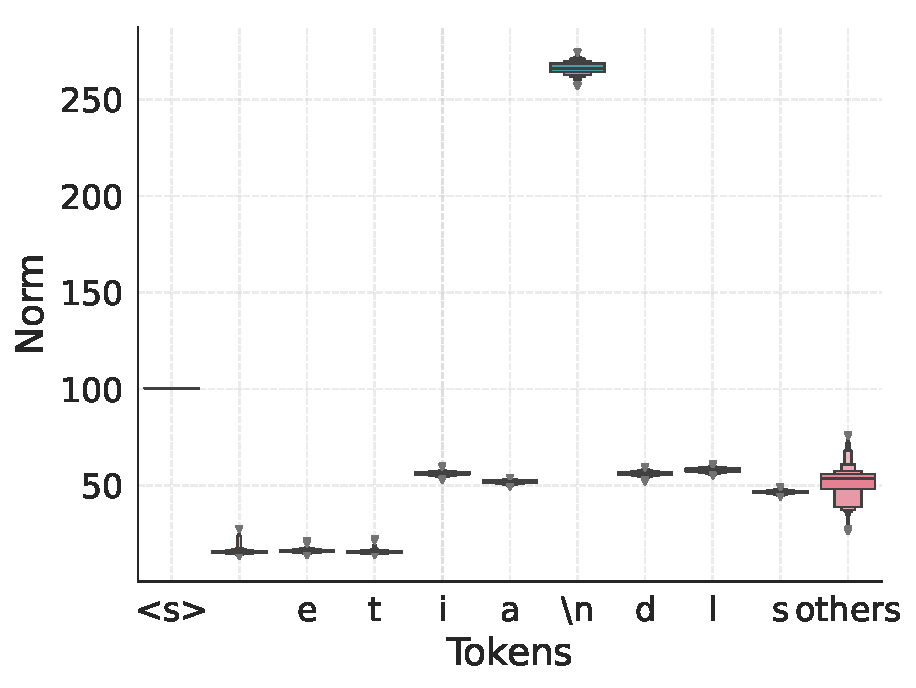
\includegraphics[width=\linewidth]{Figures/figures_pretraining/dormant_copy/dormant_copy_L3_massive.pdf}
%   \end{minipage}
%   \begin{minipage}{0.4\textwidth}
%       \centering
%       \subcaption{\small Small value states norm}
%       \label{fig:pretraining-small-value}
%       \vspace{-.2em}
%       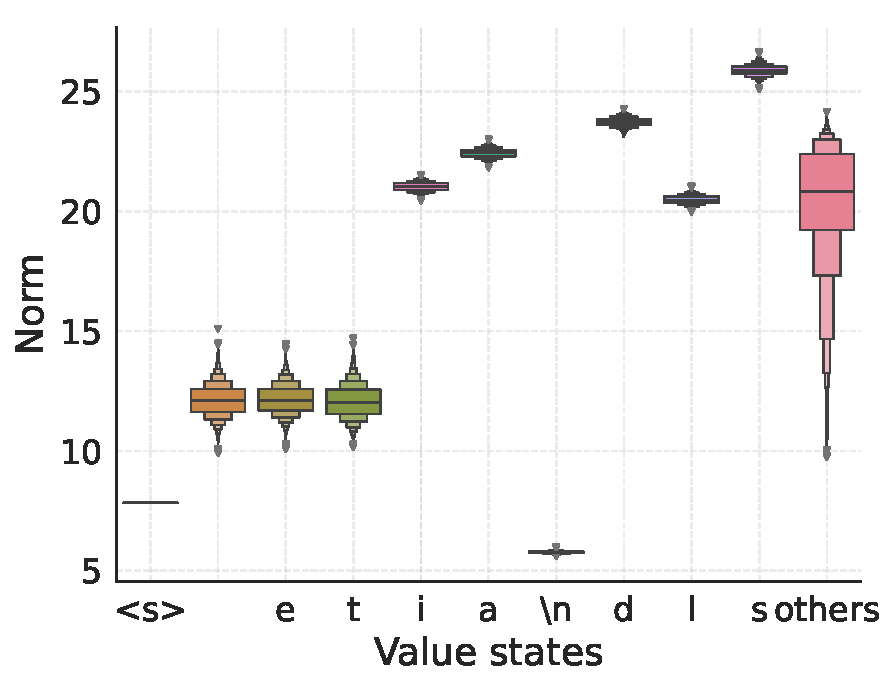
\includegraphics[width=\linewidth]{Figures/figures_pretraining/dormant_copy/dormant_copy_L3_minor.pdf}
%   \end{minipage}
%   \vspace{-1em}
%   \caption{\small \textbf{The norms of residual states and value states in the Bigram-Backcopy task.} A summary of the norm distributions of the output of layer 1 (Figure~\ref{fig:pretraining-massive-norm}) and the value states of layer 2 (Figure~\ref{fig:pretraining-small-value}) in a 3-layer transformer trained on the \textit{dormant copy} task. The \bos~token is at the left most, with three trigger tokens ` ', `t', and `e' following it. We then randomly choose six tokens and separately summarize their norm distributions. We pull all other tokens together, forming the distribution of the norms of others at the right most. Only the \bos~and the $\backslash n$ token possess remarkably large output norms and small value states norms.}
%   \label{figure:pretraining-findings-norms}
%   \vspace{-1em}
% \end{figure}

\paragraph{The \activedormant~of the attention head.} Inspired by the interpretable attention weight patterns observed, we propose the \textit{\activedormant}. For any given token, an attention head is considered \textit{active} if it makes a significant contribution to the residual state, and \textit{dormant} if its contribution is minimal. As illustrated in Figure~\ref{fig:bbm-attn}, when trained on the BB task, the attention head is active for trigger tokens and dormant for non-trigger tokens. 
% \tianyu{Link to Figure 9 more attention maps}

Figure~\ref{fig:interventions} demonstrates that the \mlp~layer is responsible for the Bigram task whereas the \attn~head takes care of the Backcopy task. When the \mlp~layer is zeroed out, the backcopy loss remains significantly better than a random guess, but the bigram loss degrades to near-random levels. Conversely, when the \attn~layer is zeroed out, the backcopy loss becomes worse than a random guess, while the bigram loss remains unaffected. This indicates that on trigger tokens, the \attn~head is active and handles the backcopy task, whereas on non-trigger tokens, the \attn~head is dormant, allowing the \mlp~layer to handle the Bigram task. We summarize the \activedormant~of the \attn~head in Claim~\ref{claim:active-dormant}.

\begin{figure}[h]
    \centering
    \begin{minipage}{0.65\textwidth}
\begin{claim}[Active-dormant mechanism]
\label{claim:active-dormant}
Attention heads of pre-trained models are often governed by the \activedormant, exhibiting two phases:
\vskip5pt
\begin{itemize}[leftmargin=2em]
\setlength\itemsep{5pt}
\item[\textup{(1)}] \textbf{Dormant phase}: On non-trigger tokens, the \attn~head assigns dominant weights to the \bos~token, adding minimal value to the residual stream and having little impact on the model’s output.
\item[\textup{(2)}] \textbf{Active phase}: On trigger tokens, the \attn~head assigns dominant attention weights to relevant context tokens, adding substantial value to the residual stream and significantly impacting the model’s output. 
\end{itemize}
\end{claim}
    \end{minipage}
    \hfill
    \begin{minipage}{0.33\textwidth}
        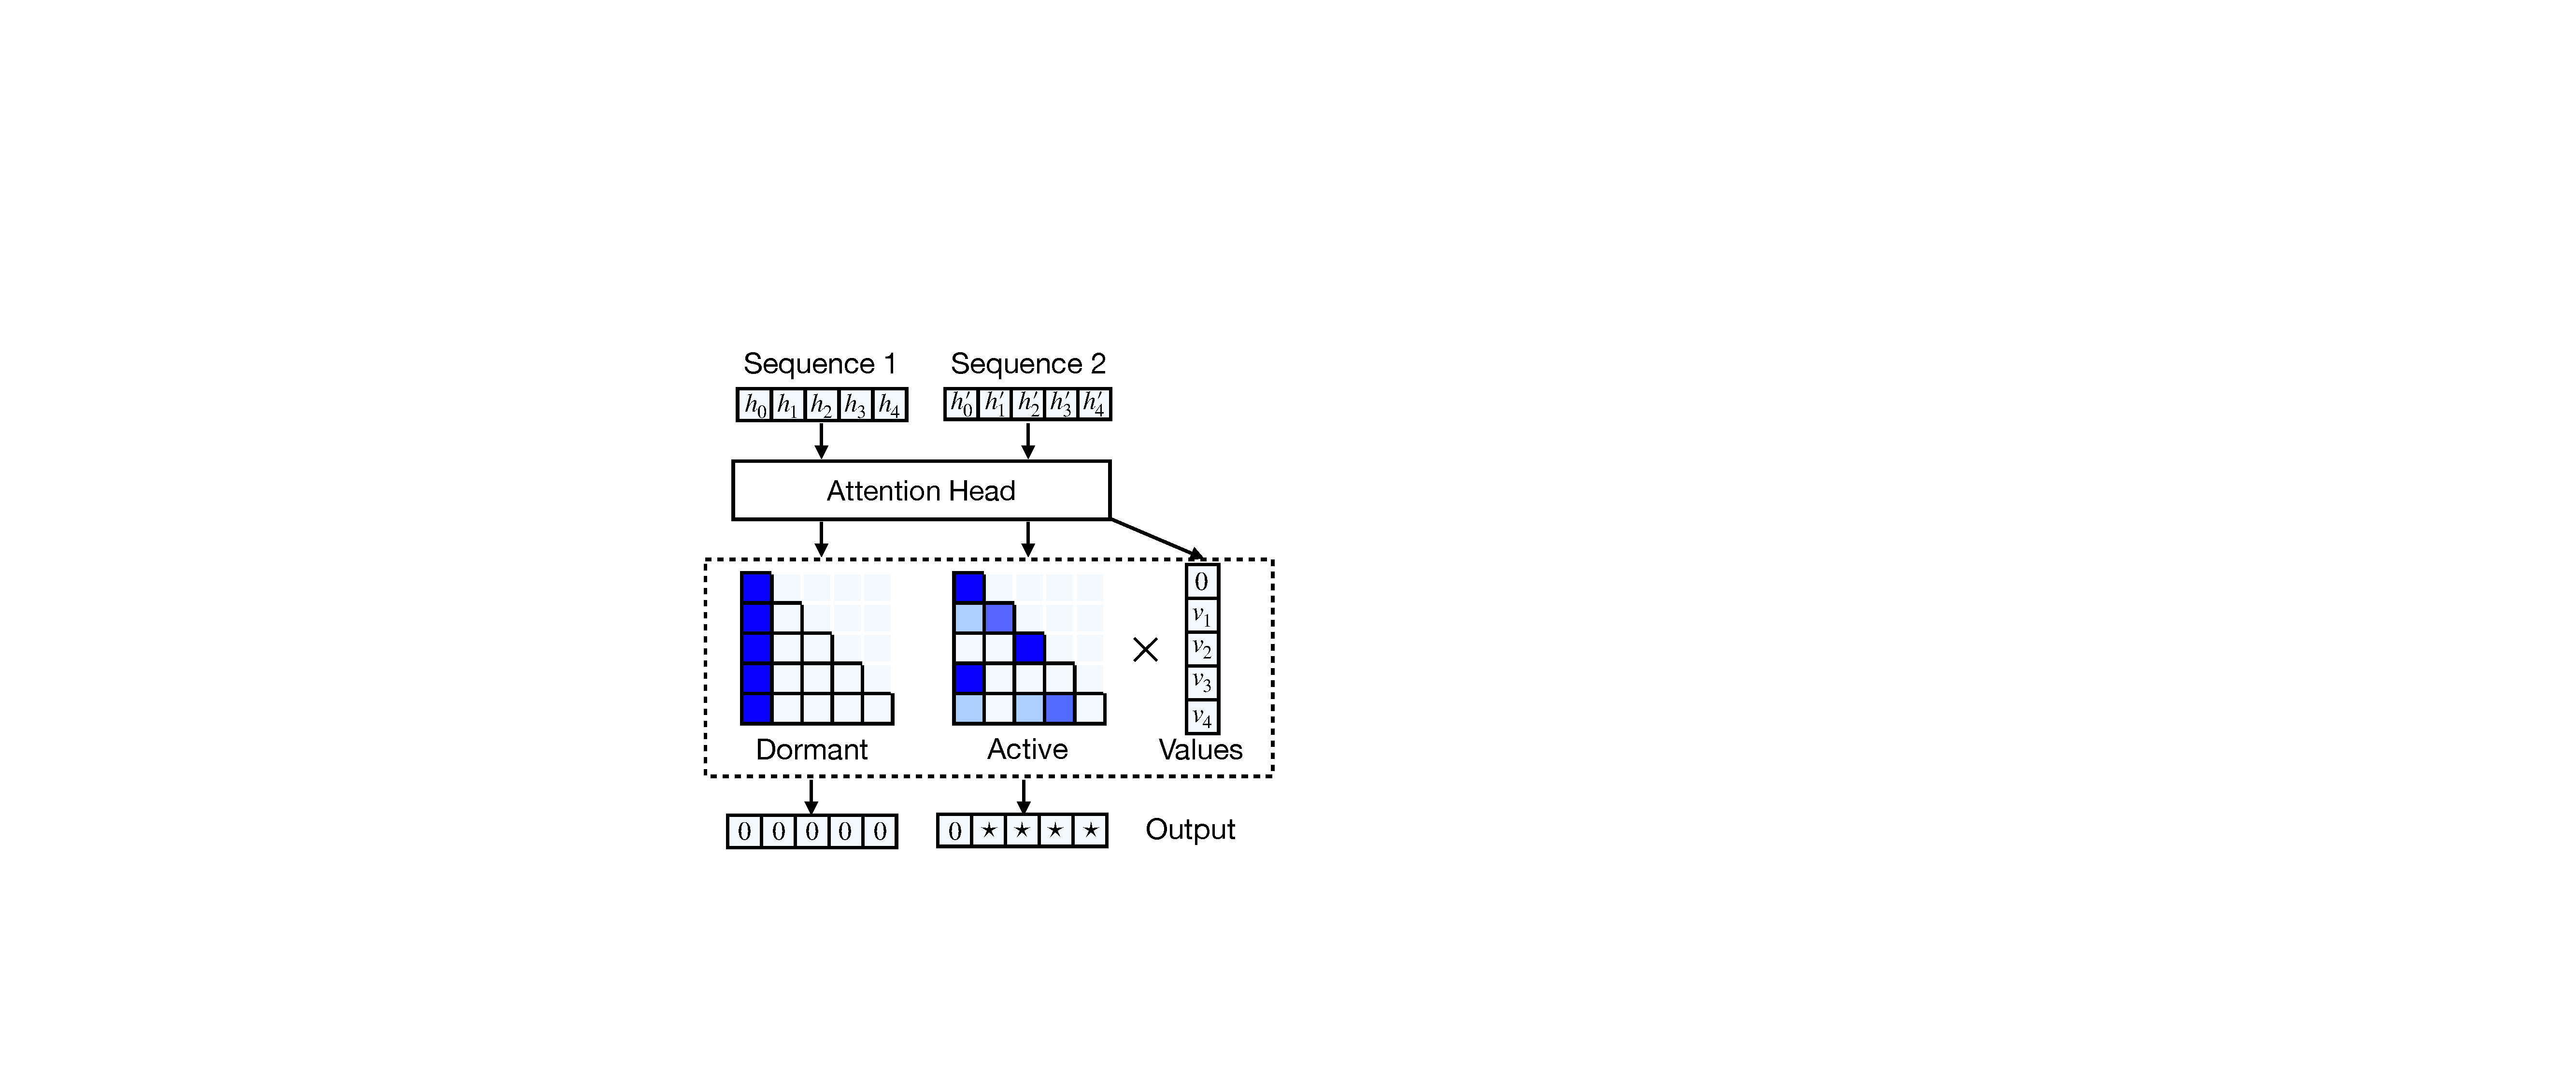
\includegraphics[width=0.89\linewidth]{Figures/illustrations/illlustrations_Part1.pdf}
        \vskip-8pt
        \caption{\small Active-dormant mechanism}
        \label{figure:illustrate-active-dormant}
    \end{minipage}%
\end{figure}

% \begin{claim}[Active-dormant mechanism]
% \label{claim:active-dormant}
% Attention heads of pre-trained models are often governed by the \activedormant, exhibiting two phases:
% \begin{itemize}[leftmargin=2em]
% \setlength\itemsep{0pt}
% \item[\textup{(1)}] \textbf{Dormant phase}: On non-trigger tokens, the \attn~head assigns dominant weights to the \bos~token, adding minimal value to the residual stream and having little impact on the model’s output.
% \item[\textup{(2)}] \textbf{Active phase}: On trigger tokens, the \attn~head assigns dominant attention weights to relevant context tokens, adding substantial value to the residual stream and significantly impacting the model’s output. 
% \end{itemize}
% \end{claim}


\begin{figure}
  \centering
  \begin{minipage}{0.37\textwidth}
      \centering
      \subcaption{\small Excess risk after interventions}
      \label{fig:interventions}
      % \vspace{-0.5cm}
      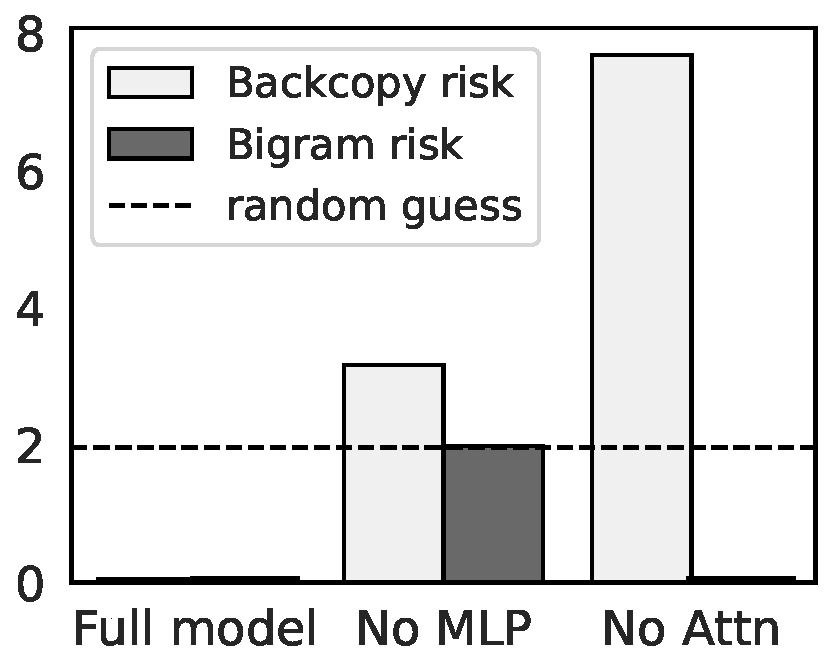
\includegraphics[width=0.94\textwidth]{Figures/BBM/interventions.pdf}
  \end{minipage}
  % \hspace{1em}
  \begin{minipage}{0.6\textwidth}
      \centering
      \subcaption{\small Training dynamics }
      \label{fig:dynamics}
    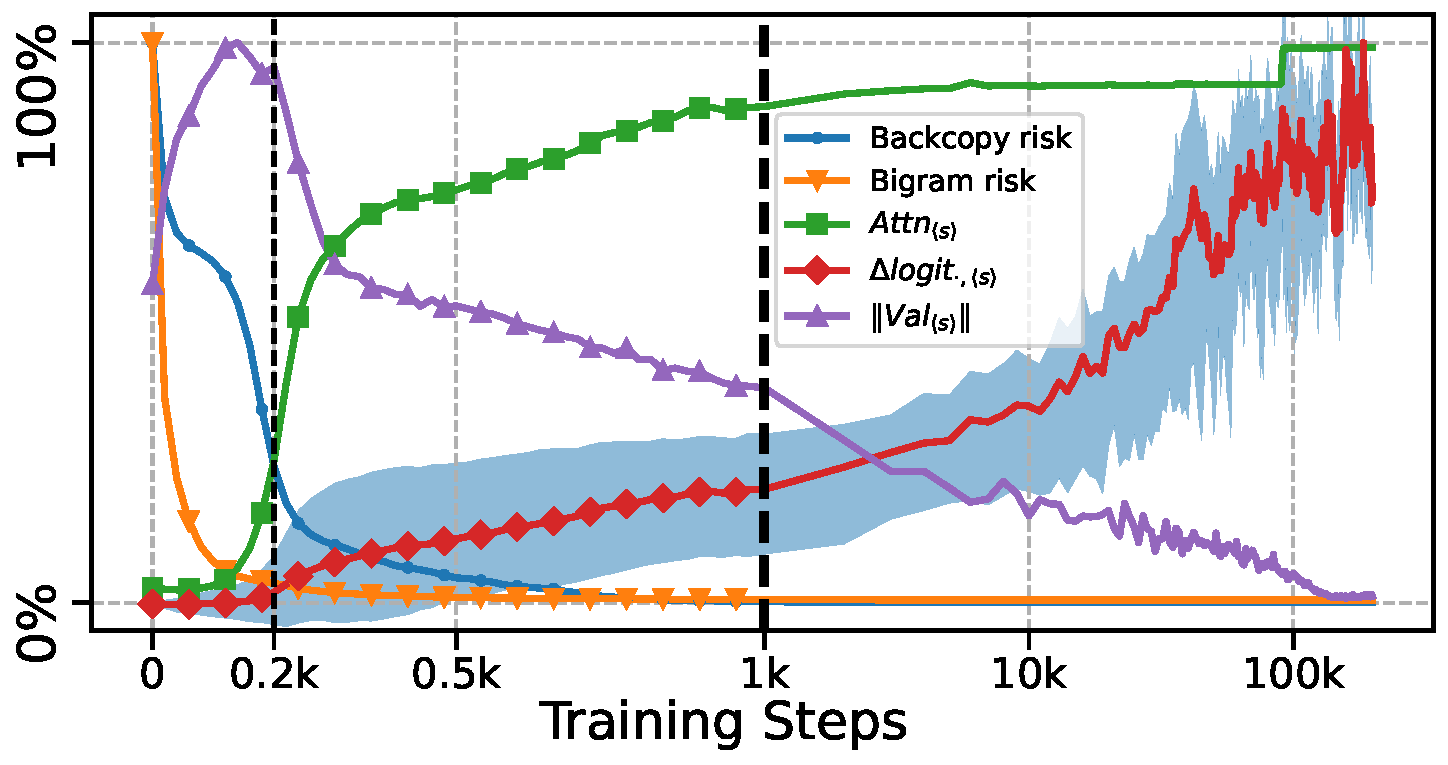
\includegraphics[width=0.87\textwidth]{Figures/BBM/dynamics_combine.pdf}
  \end{minipage}
  \hspace{-1em}
    \caption{\small \textbf{Interventions and dynamics of one-layer transformer on the Bigram-Backcopy task.}  \textit{Left (a)}: Excess risks for a one-layer model trained on the Bigram-Backcopy (BB) task under various interventions. \textit{Right (b)}: The excess risks, attention weights, attention logits, and value state norms for the \bos~token throughout the training dynamics. Each curve is rescaled to fall within a 0 to 1 range. On the right side of \textit{(b)}, the horizontal axis is logarithmically scaled. The $\Delta\text{logit}_{\cdot,\bos}$ curve represents the mean of attention logits from all given non-trigger query tokens $\tok$ on the \bos~token, normalized by the mean of attention logits for other tokens. The shaded area represents the 90\% uncertainty interval on the distribution over all non-trigger tokens. 
    % \sm{Another thinner vertical line at iteration 200. }
    % \sm{Left: Unify loss and risk. Thicker, mid line. Right: Connect left and right figure. Properly scale x. Green line $100\%$ = 1. Sparser square and triangle.} 
    % \tianyu{make 0 more obvious in full model} \tianyu{try removing markers} \sm{Why in 3(a), the backcopy risk increase so much if MLP is removed? }
    }
    \label{figure:verify-assumptions}
\end{figure}

\paragraph{The growth of attention logits on the \bos~token and the decrease in its value state norms.} Figure~\ref{fig:dynamics} illustrates the training dynamics of excess risks, attention weights, attention logits (for each token $\tok_n$ at position $n$ in the prompt, we compute $\Delta\text{logit}_{\cdot,\bos} \equiv \mathtt{mean}_{n}[\langle \query_{\tok_n}, \key_\bos \rangle - \mathtt{mean}_{i}(\langle \query_{\tok_n}, \key_{\tok_\toki}) \rangle]$, which serves as a progress measure for attention sinks), and value state norms for the \bos~token. All values are rescaled to the $0$ to $1$ range to highlight trends rather than absolute values. Both the Bigram and Backcopy excess risks decrease to nearly zero within the first 1000 steps, with the Bigram excess risk approaching zero faster than the Backcopy risk. As the Backcopy risk decreases, the attention weights on the \bos~token begin to increase, suggesting a connection between the formation of attention sinks and the backcopy function in the attention heads. After the first $1000$ steps, although both Bigram and Backcopy excess risks have nearly reached zero, the attention logits and weights on the \bos~token continue to increase, while the value state norm of the \bos~token continues to decrease. While this is an intriguing phenomenon, our next goal is to understand why the attention logits and value state norms continue to evolve toward extreme values. 



\subsection{Analysis of a minimally-sufficient transformer architecture}
\label{sec:simple-model}


\begin{figure}[t]
    \centering
    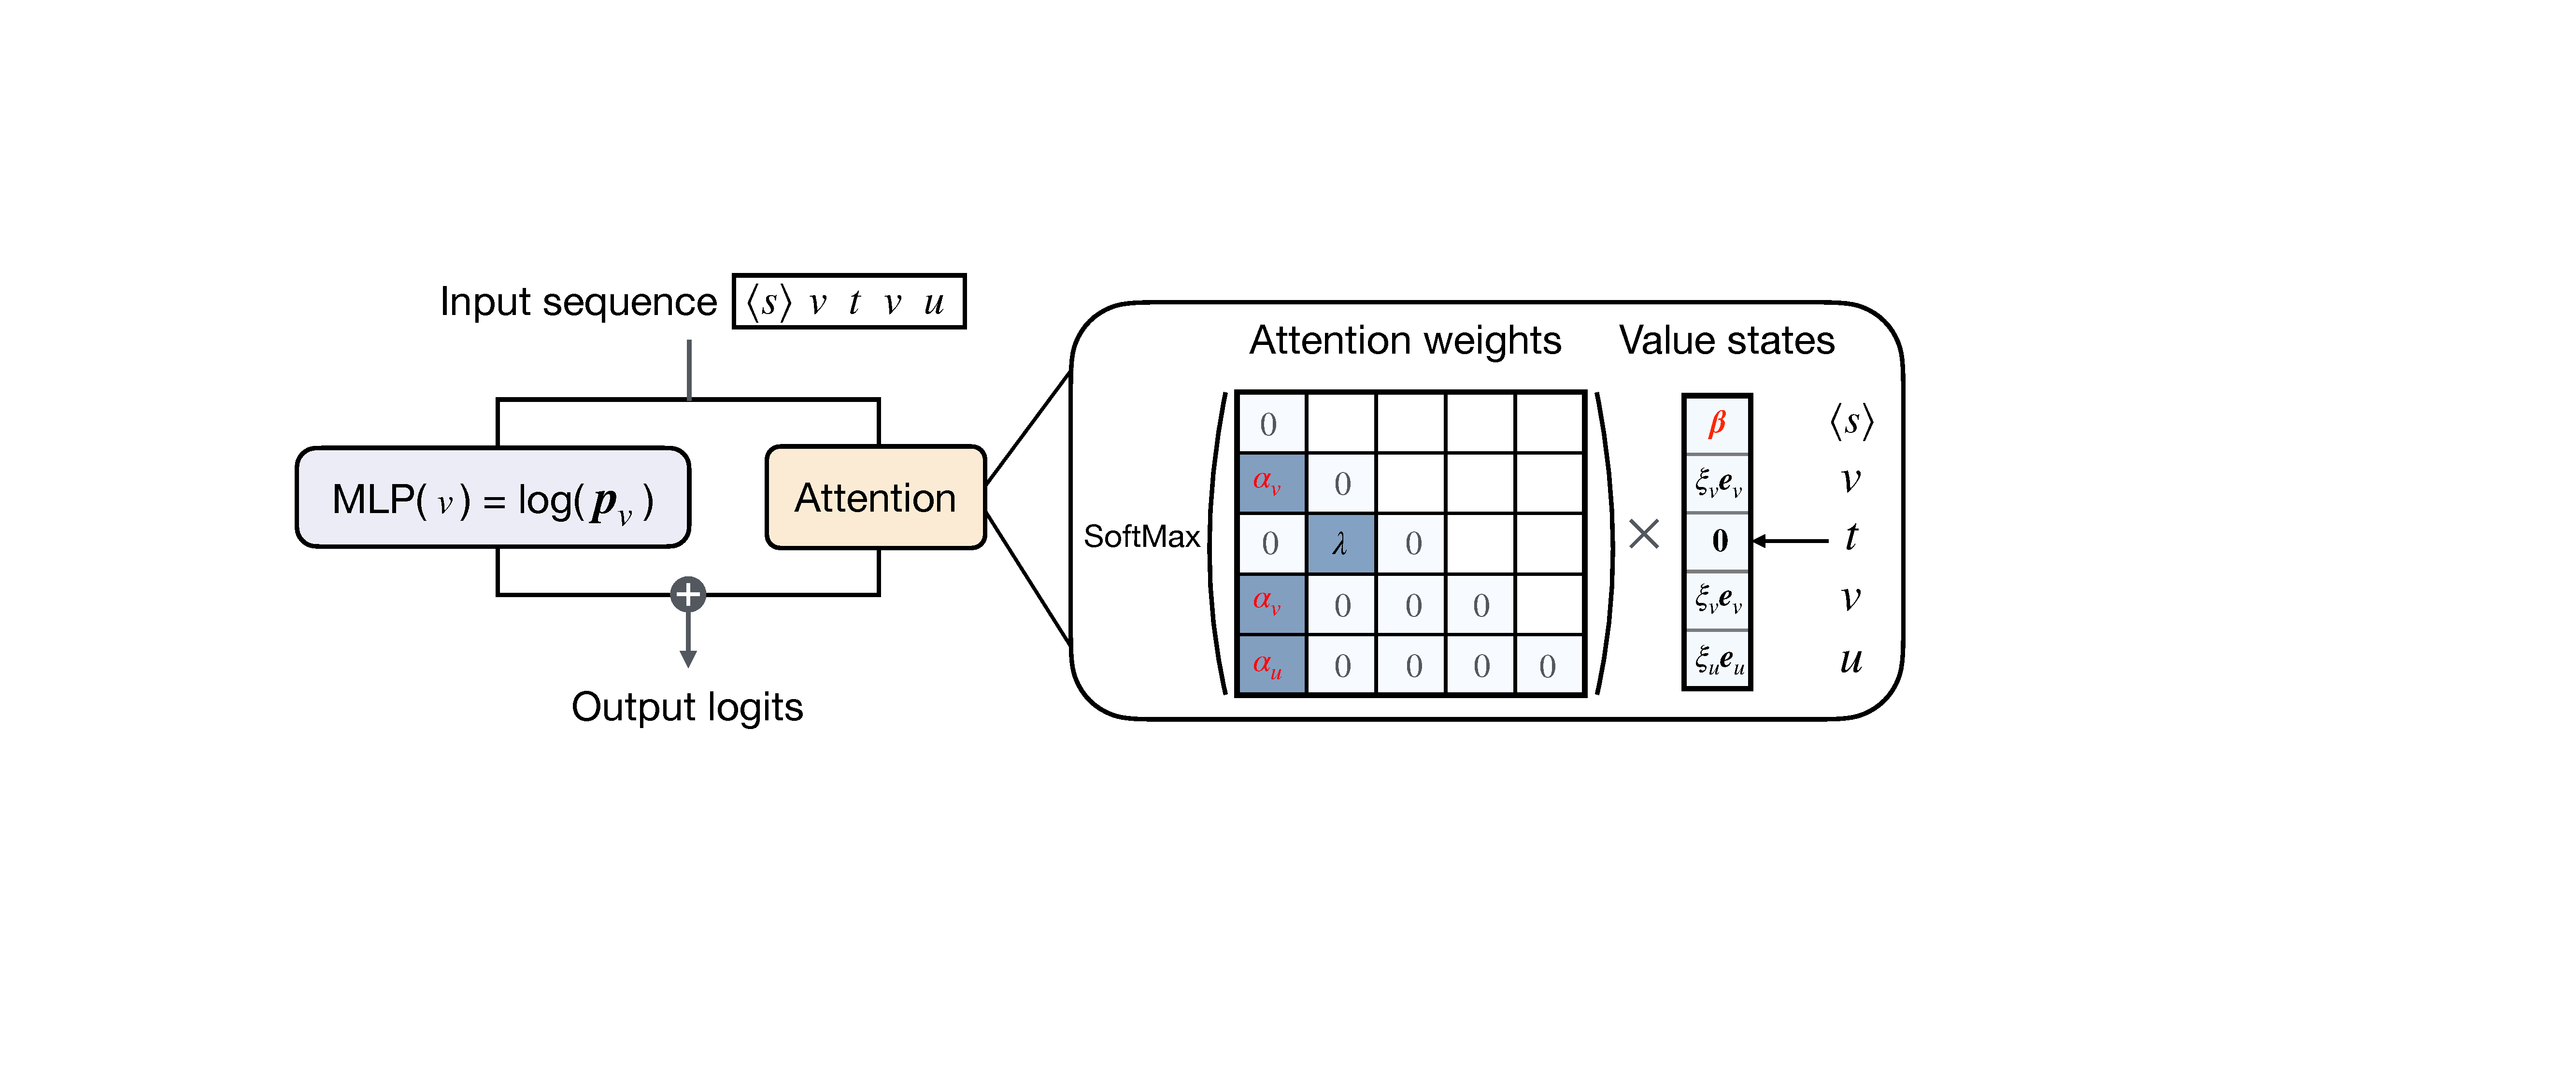
\includegraphics[width=0.7\linewidth]{Figures/BBM/SimpleModel.pdf}
    \caption{\small \textbf{Simplified transformer architecture.} The output logits are computed by summing the contributions from both the \mlp~layer and the \attn~head. The predicted probabilities are obtained by applying the SoftMax function to these output logits. The \mlp~layer is assumed to provide the Markov transition probabilities for non-trigger tokens, while the \attn~head is parameterized by attention logits and value states, as described in Eq.~(\ref{eqn:simplification_TF_1}), (\ref{eqn:simplification_TF_2}), and (\ref{eqn:simplification_TF_3}). Additionally, the trainable variables, denoted by $(\vecsink,\vecvalue) \in \R^V \times \R^V$, represent the attention logits and value states of the \bos~token.}
    \label{figure:simple-model}
\end{figure}

In this section, we analyze the training dynamics of transformers on the BB task, focusing on a simplified architecture that retains the attention sinks and value-state-drains phenomena. We analyze the regime when the Bigram transition probability is fully learned, and the Backcopy task is partially learned (i.e., after step $200$ in Figure~\ref{fig:dynamics}), and we focus on the dynamics of the attention logits and value states. Readers who are more interested in the results than the theoretical analysis can skip the detailed analysis and proceed directly to the statement of the mutual reinforcement mechanism in Claim~\ref{claim:mutual-reinforcement}. 

Let $\vocab$ (of size $V$) denote the set of all tokens excluding the $\bos$ token, and let $\cT$ represent the set of all trigger tokens. For any  $\tok \in \vocab$, we define $\transition_{\tok\tokk}=\transit(\tokk|\tok)$ as the next-token Markov transition probability, and $\bm{\transition}_v = (p_{v1}, \ldots, p_{vV})^\top \in \Delta(\cV)$ as the transition vector in the simplex. The embedding map is denoted by $\embd: [n] \times \cV \to \R^D$, where for a token $v \in \cV$ at position $i \in [n]$, the embedded vector is $\embd_i(\tok)$. The \bos~token always appears at position $0$, and we denote its embedding vector by $\embd(\bos)$. For simplicity, we abuse the notation and use the sequence itself, $[\bos, \tok_1, \ldots, \tok_n]$ where $\{ \tok_{k} \}_{k \in [n]} \subseteq \cV$, to represent the embedding of the sequence. 

Given an input sequence $\bH = [\bos, v_{1:n}] \in \R^{D \times (n+1)}$ with \bos~as the zeroth token, we define the predicted probability of the next token as $\softmax(\TF(\bH)_n)$, where $\TF(\bH)_n \in \R^D$ is the last column of $\TF(\bH) \in \R^{D \times (n+1)}$, defined as
\begin{equation}\label{eqn:simplified_transformer}
\TF(\cdot) = \attn(\cdot) + \mlp(\cdot),~~\attn(\bH) = \bV \bH \softmax(\mask(\bH^\top \bK^\top \bQ \bH ) ),~~ \mlp(\bH) = \bW_2 \relu( \bW_1 \bH).
\end{equation}
The simplified transformer architecture $\TF$ is a parallel summation of the $\attn$ head and the $\mlp$ layer, with no layer normalization. This parallel summation is a reasonable simplification, as sequential $\attn$ and $\mlp$ layers can effectively simulate parallel $\attn$ and $\mlp$ operations. Notice that we have redefined the notations of $\attn$ and $\mlp$ in this section, which are simplified versions of Eq.~(\ref{eqn:attention_head_prelim}) and (\ref{eqn:MLP_layer_prelim}). %The parallel simplification in Eq.~\eqref{eqn:simplified_transformer} also fits the intervention results in Figure~\ref{fig:interventions}, which shows that the $\attn$ and $\mlp$ layers in sequential structure have separable functions.


\paragraph{Simplification and reparameterization of the model.} To simplify the analysis of the training dynamics, we further reduce the model by restricting the $(\bK, \bQ, \bV, \bW_1, \bW_2)$ matrices to follow the patterns observed in the later training stages (i.e., after step 200 of the training in \Cref{fig:dynamics}). 
\begin{itemize}[leftmargin=2em]
\setlength\itemsep{0pt}
\item \textit{Restricted Attention Pattern}. Based on the intuition from \Cref{fig:bbm-attn}, we know that eventually only a few attention logits are non-trivial. Thus, we assume that the model has learned the attention pattern by this stage (which is reasonable given that the Backcopy risk is already small after step 200 in \Cref{fig:dynamics}). We parameterize the attention logits on the $\bos$ key-token as $(\sink_{\bos}; \sink_{v_1}; \ldots; \sink_{v_n})$, restrict the attention logits for any trigger query-token to $(0, \ldots, \lambda, 0)$ (where the second-to-last coordinate is $\lambda$), and set all other logits to zero. Specifically, we restrict:
\begin{equation}\label{eqn:simplification_TF_1}
\begin{aligned}
&~\embd(\bos)^\top \bK^\top \bQ \cdot \embd_i(\tok) =\sink_\tok \cdot 1 \{ v \not\in \cT \}~~~\text{for } \tok\in\vocab, i \in [n], \\
&~ \embd_i(\bar \tok)^\top \bK^\top \bQ \cdot \embd_j(\tok) = \lambda \cdot 1\{ \tok \in \cT, i = j-1 \} ~~~\text{for } \tok, \bar \tok \in \cV, i, j \in [n]. 
\end{aligned}
\end{equation}
Notice that this naturally implies $\sink_v = 0$ for $v \in \cT$. 
\item \textit{Restricted Value Pattern}. At later stages of the training dynamics, we observe that the value states for each token are nearly a scaled version of the one-hot encoding vector. We assume this observed pattern and parameterize the value state of $\tok$ by $\xi_\tok \bm{e}_{\tok} \in \R^V$. For the \bos~token, we parameterize its value state by $\vecvalue \in \R^{V}$. Specifically, we restrict
\begin{equation}\label{eqn:simplification_TF_2}
\begin{aligned}
&~ \bV \cdot \embd(\bos)  = \vecvalue \in \R^{V}, \\
&~ \bV \cdot \embd_i(\tok)  = \xi_\tok \bm{e}_\tok \in \R^{V},  ~~~\text{with $\xi_\tok=0$ for $\tok\in\cT$, and $\xi_\tok\geq 0$ for $\tok\in\vocab\setminus\cT$.} 
\end{aligned}
\end{equation}
\item \textit{MLP Layer Perfectly Predicts the Transition Probability}. Notice that the \mlp~layer handles the Bigram task. By step 200 in \Cref{fig:dynamics}, the Bigram risk has nearly vanished. Therefore, we assume that the $\mlp$ layer outputs the Markov transition probabilities $\bm{\transition}_{\tok}$ for non-trigger tokens $\tok$, and zero for trigger tokens. Specifically, we restrict: 
\begin{equation}\label{eqn:simplification_TF_3}
\mlp(\embd_i(\tok)) = \log \bm{\transition}_v \cdot 1\{ \tok \not\in \cT  \} ~~~ \text{for } \tok \in \vocab. 
\end{equation}
\end{itemize}
% Let $\vocab$ (of size $V$) denote the set of all tokens except the $\bos$ token, and $\cT$ denote the set of all trigger tokens. Given any $\tok \in \vocab$, we denote $\transition_{\tok\tokk}=\transit(\tokk|\tok)$ to be the next token Markov transition probability, and $\bm{\transition}_v = [p_{v1}, \ldots, p_{vV}] \in \Delta(\cV)$ be the row vector in the simplex. We assume that the tokens are embedded into $(V + 1)$-dimensional space using one-hot encoding, and for notation simplicity, we abuse $v \in \{ \bos \} \cup \cV$ to stand for its one-hot encoding vector $\bm{e}_v \in \R^{V+1}$, which is a row vector. 

% Given an input sequence $\bH = [\bos; v_{1:n-1}; v] \in \R^{(n+1) \times D}$ with \bos~as the zeroth token, we take the predicted probability of the next token to be $\softmax(\TF(\bH)_n)$, where $\TF(\bH)_n \in \R^D$ is the last row of $\TF(\bH) \in \R^{(n+1) \times D}$. The simplified transformer architecture $\TF$ is a parallel summation of the attention head and the MLP layer, without layer normalization: $\TF(\bH) = \attn(\bH) + \mlp(\bH)$, where the attention head and MLP layer are defined as\footnote{These are simplifications of Eq.~(\ref{eqn:attention_head_prelim}) and (\ref{eqn:MLP_layer_prelim}), but we abuse the notation and reuse $\attn$ and $\mlp$. }
% \[
% \attn(\bH) = \softmax(\mask(\bH \bQ \bK^\top \bH^\top )) \bH \bV \in \R^{(n+1) \times D},~~~ \mlp(\bH) = \relu(\bH \bW_1) \bW_2.
% \]

% In the following, we make assumptions on the $(\bK, \bQ, \bV, \bW_1, \bW_2)$ matrices to simplify the analysis of training dynamics. By the intuition from \Cref{fig:bbm-attn}, we know that eventually, there are only a few attention logits that are non-trivial, and hence we assume that the model has already learned the attention pattern (this is a reasonable assumption when we are at step 200 of \Cref{fig:dynamics}, since the Backcopy risk is already small). We thus parameterize attention logits on the $\bos$ key-token by $(\sink_{\bos}; \sink_{v_1}; \ldots; \sink_{v_n})$, parameterize the attention logits on any trigger query-token by $(0, \ldots, \lambda, 0)$ where the second-to-last coordinate is $\lambda$, and assume all other logits are zero. That is, we assume \sm{Redefine $\query$ in appendix}
% \begin{equation}
% \begin{aligned}
% &~\tok \bQ \bK^\top \bos^\top =\sink_\tok \cdot 1 \{ v \not\in \cT \}~~~\text{for } \tok\in\vocab, \\
% &~ \tok \bQ \bK^\top (v')^\top = \lambda \cdot 1\{ \tok \in \cT, \tok' \text{ is the former token of } \tok \} ~~~\text{for } \tok, \tok' \in \cV. 
% \end{aligned}
% \end{equation}
% By the patterns of the value matric observed in the training dynamics, we assume that the value state of $\bos$ is $\vecvalue \in \R^V$, and the value state of each non-trigger token $\tok$ is a one-hot encoding vector $\bm{e}_\tok$ multiplied by $\xi_\tok \geq 0$. That is, 
% \begin{equation}
% \begin{aligned}
% \bos \bV = \vecvalue \in \R^{V+1}, ~~~ \tok \bV = \xi_\tok \bm{e}_\tok \in \R^{V+1}  ~~~\text{with $\xi_\tok=0$ for $\tok\in\cT$, and $\xi_\tok\geq 0$ for $\tok\in\vocab\setminus\cT$.}
% \end{aligned}
% \end{equation}

% Since the \mlp~layer handles the Bigram task, we assume that the $\mlp$ layer outputs the Markov transition probabilities $\bm{\transition}_v$ on non-trigger tokens $v$ and zero on trigger tokens, i.e.,
% \[
% \mlp(\tok) = \log \bm{\transition}_v \cdot 1\{ \tok \not\in \cT  \} ~~~ \text{for } \tok \in \vocab. 
% \]
% Figure~\ref{figure:simple-model} illustrates this simplified transformer architecture. %These assumptions are summarized in the following equations: \sm{Be more careful in justifying these assumptions.} \sm{Mid priority}
% \begin{equation}\label{eqn:simplification_TF}
% \begin{aligned}
% &~ \mlp(\tok) = \log \bm{\transition}_v \cdot 1\{ \tok \not\in \cT  \} ~~~ \text{for } \tok \in \vocab,\\
% &~\langle \query(\tok), \key(\bos) \rangle =\sink_\tok \cdot 1 \{ v \not\in \cT \}~~~\text{for } \tok\in\vocab, \\
% &~\langle \query(\tok), \key(\tok') \rangle = \lambda \cdot 1\{ \tok \in \cT, \tok' \text{ is the former token of } \tok \} ~~~\text{for } \tok, \tok' \in \cV, \\
% &~ \vall(\tok) = \xi_\tok \bm{e}_\tok  ~~~\text{with $\xi_\tok=0$ for $\tok\in\cT$, and $\xi_\tok\geq 0$ for $\tok\in\vocab\setminus\cT$.}
% \end{aligned}
% \end{equation}

These reparameterizations are illustrated in Figure~\ref{figure:simple-model}. Theorem~\ref{thm:construction} establishes the existence of a transformer architecture that satisfies the restrictions and reparameterizations outlined above. Furthermore, this restricted transformer can generate the ground-truth transitions of the BB model when certain parameters diverge. 
\begin{theorem}[Existence of reparameterization that solves the BB task; informal]\label{thm:construction}
For any parameters $(\vecsink \in \R^{V}, \vecvalue \in \R^V, \bm{\xi} \in \R^V, \lambda \in \R)$, there exists a one-layer transformer as described in (\ref{eqn:simplified_transformer}) with weight matrices $(\bQ, \bK, \bV, \bW_1, \bW_2)$ such that Eq. (\ref{eqn:simplification_TF_1}), (\ref{eqn:simplification_TF_2}), and (\ref{eqn:simplification_TF_3}) hold. Furthermore, there exists a sequence of parameters where $\min_{v \in \vocab} \sink_v \to\infty$, $\min_{v \in \vocab} \xi_v \to\infty$, $\lambda\to \infty$, and $\vecvalue=0$, such that this transformer generates the ground-truth transitions of the BB model in the limit. %\tianyu{describe the def of ground-truth transitions of the BB model} \tianyu{assume the embedding satisfy...}
\end{theorem}
The formal statement and proof of \Cref{thm:construction} are provided in Appendix~\ref{app:proof-construction}. 

% \sm{I am here.} We make further simplifications on the loss function. Given a non-trigger token at position $n$, assume $W=\sum_{i=1}^n \exp \query_n^\top \key_i $. Assume that $W=\sum_{\tokk=1}^\vocabsize W_\tokk$, with each $W_\tokk$ corresponds to the summations from . We assume that they are fixed values and do not depend on the position $n$. %In reality $W\approx N/2$, which is half of the total sequence length. Since token $\tokk$ takes a proportion $\stable_\tokk$ in the stable distribution, $W_\tokk \approx \stable_\tokk W$ on average. 
\paragraph{Dynamic analyses of the reparameterized model.} To analyze the later stage training dynamics, we adopt the reparameterization given in Eq.~(\ref{eqn:simplification_TF_1}), (\ref{eqn:simplification_TF_2}), and (\ref{eqn:simplification_TF_3}) as our assumption. We further define $\mass_{\tokk} = \sum_{i = 1}^n 1\{ \tok_i = \tokk \}$, $\bm{\mass} = (\mass_1, \ldots, \mass_V)$, and $\mass = \sum_{\tokk \in \vocab} \mass_{\tokk} = n$. Substituting these into Eq.~\eqref{eqn:simplified_transformer}, for a non-trigger token $v \in \cV \setminus \cT$, the output of the attention layer with input sequence $\bH = [\bos, v_{1:n-1}, v]$ is given by 
\begin{equation}\label{eqn:q}
\TF(\bH)_n = \log \bm{\transition}_v + \frac{e^{\sink_\tok}}{e^{\sink_\tok} + \mass} \vecvalue + \sum_{\tokk=1}^{\vocabsize} \frac{\mass_\tokk \xi_\tokk}{e^{\sink_\tok} + \mass} \cdot \bm{e}_\tokk.
\end{equation}
Therefore, for the non-trigger token $\tok$, the cross-entropy loss between the true Markov transition $\bm{\transition}_\tok$ and the predicted transition $\softmax(\TF(\bH)_n)$ is given by
\begin{equation}\label{eqn:loss_single}
\loss_\tok(\sink_\tok, \vecvalue) = \sum_{\tokk=1}^\vocabsize \transition_{\tok\tokk}\Big\{ \log \Big[ \sum_{\toki=1}^\vocabsize \transition_{\tok\toki} \exp\Big(\frac{e^{\sink_\tok}\ivalue_\toki+\mass_\toki\xi_\toki}{e^{\sink_\tok}+\mass}\Big) \Big] - \frac{e^{\sink_\tok}\ivalue_\tokk+\mass_\tokk\xi_\tokk}{e^{\sink_\tok}+\mass} - \log \transition_{\tok\tokk} \Big\}.
\end{equation}
For simplicity, we neglect the loss on trigger tokens and assume that $(\{ \mass_i \}_{i \in [V]}, \mass)$ remain fixed across different positions in the input sequences.\footnote{We note that \cite{reddy2023mechanistic} makes a similar simplification in analyzing induction heads.} We then consider the total loss as the average of the losses on each non-trigger token, weighted by its proportion in the stable distribution $\{\pi_v\}_{v \in \vocab}$, given by
\begin{equation}\label{eqn:total_loss}
\textstyle \loss(\vecsink,\vecvalue) = \sum_{\tok \in \vocab \setminus \cT} \stable_\tok \cdot \loss_\tok(\sink_\tok, \vecvalue).
\end{equation}
We assume that $\bm{\xi}$ and $\lambda$ are fixed, and that $\vecsink$ (the attention logits of the \bos~token) and $\vecvalue$ (the value state norms of the \bos~token) are trainable variables, as we are interested in the dynamics of the attention logits and value state norm for the \bos~token. The following theorem illustrates the logarithmic growth of the attention logits $\vecsink$, the shrinkage of value states $\vecvalue$, and the stable phase of these two variables.
% \tianyu{change the summation notation in the proof.}
\begin{theorem}\label{thm:main}
Consider the gradient flow of the loss function $\loss(\vecsink, \vecvalue)$. Assume $\xi_\tok \ge 0$ for any $\tok$ and $\stable_\tok > 0$ for any $\tok\in\vocab$, and $\{ \mass_i \cdot \xi_i \}_{i \in \vocab}$ are not all equal. 
\begin{itemize}[leftmargin=2em]
\setlength\itemsep{0pt}
    \item[\textup{(a)}] (Attention logits grow logarithmically, reinforced by small value states) Fix $\vecvalue= \beta \cdot \bm{1}$ for a constant $\beta$, and consider the gradient flow over $\vecsink$. With any initial value $\vecsink(0)$, there exists $\bm{r}(t)$ with norm uniformly bounded in time, such that 
    \begin{equation}
    \textstyle \vecsink(t) = \frac{1}{2} \log t \cdot \bm{1} + \bm{r}(t).\end{equation}
    \item[\textup{(b)}] (Value state shrinks to a small constant vector, reinforced by large attention logits) Fix $\vecsink = \sink \cdot \bm{1}$ for a constant $\sink$, define $\bar{\ivalue}(0) = V^\inv[\sum_{\tok} \ivalue_\tok(0)]$ and $\meanvalue=\vocabsize^\inv[\sum_{\tok} \mass_\tok \xi_\tok]$. Consider the gradient flow over $\vecvalue$. As $t \to \infty$, we have
    \begin{equation}\vecvalue(t) \to \vecvalue^\star = [\bar\ivalue(0)+e^{-\sink} \meanvalue] \cdot \bm{1} - e^{-\sink} \cdot \bm{\mass}\circ \bm{\xi}.\end{equation}
    \item[\textup{(c)}] (Stable phase: Sink-logits concentration) Consider the gradient flow over the variables $(\vecsink, \vecvalue)$. Any vector of the following form
    \begin{equation}\vecsink = \sink \cdot \bm{1}, \quad \vecvalue = c \cdot \bm{1} - e^{-\sink} \cdot \bm{\mass} \circ \bm{\xi},  ~~~ \sink, c\in\R \end{equation}
     is a stationary point. These are all global minimizers of $\loss(\vecsink,\vecvalue)$.
\end{itemize}
\end{theorem}
The proof of Theorem~\ref{thm:main} is provided in Appendix~\ref{app:proof-main-3}, \ref{appsec:proof-main-1}, and \ref{appsec:proof-main-2}. We offer two key remarks: (1) As $\sink_\tok\to\infty$, a Taylor expansion of the gradient $\partial \loss/\partial \sink_\tok$ suggests that $\mathrm{d}\sink_\tok/\mathrm{d}t \propto \exp(-2 \sink_\tok)$, which leads to the logarithmic growth of $\sink_\tok$. Similar logarithmic growth has been reported in the literature under different setups \citep{tian2023scan,zhu2024towards};
(2) The stable phase described in Theorem~\ref{thm:main}(c) seems to imply that the system can remain stable without attention sinks, as it does not require $\sink$ to be large. However, in practice, models trained on the BB task tend to converge to a stable phase where $\sink$ is relatively large. 

% (2) For a fixed $\vecsink=\sink\bm{1}$, under additional assumptions on the initial value $\vecvalue(0)$, we can prove a linear convergence for $\vecvalue$. 
% \tianyu{We expect LLMs to converge to the stable phase outlined in Theorem~\ref{thm:main} as well.}
% Revisiting Figure~\ref{fig:attention_logits_random}, which shows attention logits in Llama 2-7B, the attention logits on the \bos~token appear identical. 
% Thus, we expect LLMs to converge to the stable phase outlined in Theorem~\ref{thm:main} as well.

\paragraph{The formation of attention sinks and value-state drains.} Below, we explain how Theorem~\ref{thm:main} reveals the \textit{mutual reinforcement mechanism} behind the formation of attention sinks and value-state drains.  
\begin{itemize}[leftmargin=2em]
\item[(a)] When the value states of the \bos~token are small and constant, $\vecvalue = \ivalue \cdot \bm{1}$, Theorem~\ref{thm:main}(a) shows that the attention logits on the \bos~token $\vecsink(t) \approx \sink(t) \bm{1}$  for $\sink(t) = (1/2) \log t$, grow logarithmically. This demonstrates that the presence of a small constant value state ($\vecvalue = \ivalue \cdot \bm{1}$) reinforces the formation of attention sinks ($\vecsink(t) \approx \sink(t) \cdot \bm{1}$ for $\sink(t)$ increases logarithmically). 
\item[(b)] When the attention logits of the \bos~token are large and constant, $\vecsink = \sink \cdot \bm{1}$ for $\sink \to \infty$, Theorem~\ref{thm:main}(b) shows that the value states of the \bos~token $\vecvalue(t) \to \bar{\ivalue}(0) \cdot \bm{1}$. Starting with a random Gaussian initialization for $\vecvalue(0)$, we have $\|\vecvalue(t)\|_2 \approx \|\bar{\ivalue}(0) \cdot \bm{1}\|_2 \approx \|\vecvalue(0)\|_2 / \sqrt{V}$, where $V$ is the vocabulary size, typically large. This indicates that attention sinks ($\vecsink = \sink \cdot \bm{1}$ for large $\sink$) reinforces the formation of value-state drains ($\vecvalue(t) \to \ivalue \cdot \bm{1}$ for small $\ivalue$). 
\item[(c)] In the later stages of the dynamics, both the attention logits and value states of the \bos~token stabilize, as described in~\ref{thm:main}(c). The attention logits remain constant at $\vecsink = \sink \cdot \bm{1}$ with large $\sink$, while the value states become small, $\vecvalue = [\bar\ivalue(0)+e^{-\sink} \meanvalue] \cdot \bm{1} - e^{-\sink} \cdot \bm{\mass}\circ \bm{\xi}$. 
\end{itemize}



% \begin{claim}[Mutual reinforcement mechanism]\label{claim:mutual-reinforcement}
% For any attention head given a specific prompt, if the model can accurately predict the next token without using the attention head, but adding any value state from previous tokens—except for certain special tokens—worsens the prediction, the attention head will become dormant, forming an attention sink at those special tokens. Dynamically, this arises from a mutual reinforcement between attention sinks and value-state drains:
% For any attention head given a specific prompt, if the model can accurately predict the next token without using the attention head, but adding any value state from previous tokens worsens the prediction, the attention head will become dormant, forming an attention sink. This leads to a mutual reinforcement between attention sinks and value-state drains:

Based on these theoretical insights, we summarize the dynamical mechanism underlying attention sinks and value-state drains: For any attention head given a specific prompt, if the model can accurately predict the next token without using the attention head, but adding any value state from previous tokens—except for certain special tokens—worsens the prediction, the attention head will become dormant, forming an attention sink at those special tokens. This phenomenon is induced by the mutual reinforcement mechanism, as described below: 
\begin{figure}[h]
    \centering
    \begin{minipage}{0.68\textwidth}
    \begin{claim}[Mutual reinforcement mechanism]\label{claim:mutual-reinforcement}
Dynamically, attention sinks and value-state drains arise through mutual reinforcement:
\begin{itemize}[leftmargin=2em]
\setlength\itemsep{0pt}
    \item[\textup{(a)}] The SoftMax mechanism shifts attention weights towards tokens that exhibit value-state drains, reinforcing these tokens as attention sinks. 
    \item[\textup{(b)}] Attention sinks on these extreme tokens further suppress their value states, reinforcing their role as value-state drains. 
    \item[\textup{(c)}] The mutual reinforcement stabilizes when all non-trigger tokens have large, nearly identical attention logits on the extreme token. 
\end{itemize} 
Due to the causal mask, the training dynamics favor the \bos~token as the extreme token. 
\end{claim}
    \end{minipage}
    ~~~~
    \begin{minipage}{0.28\textwidth}
        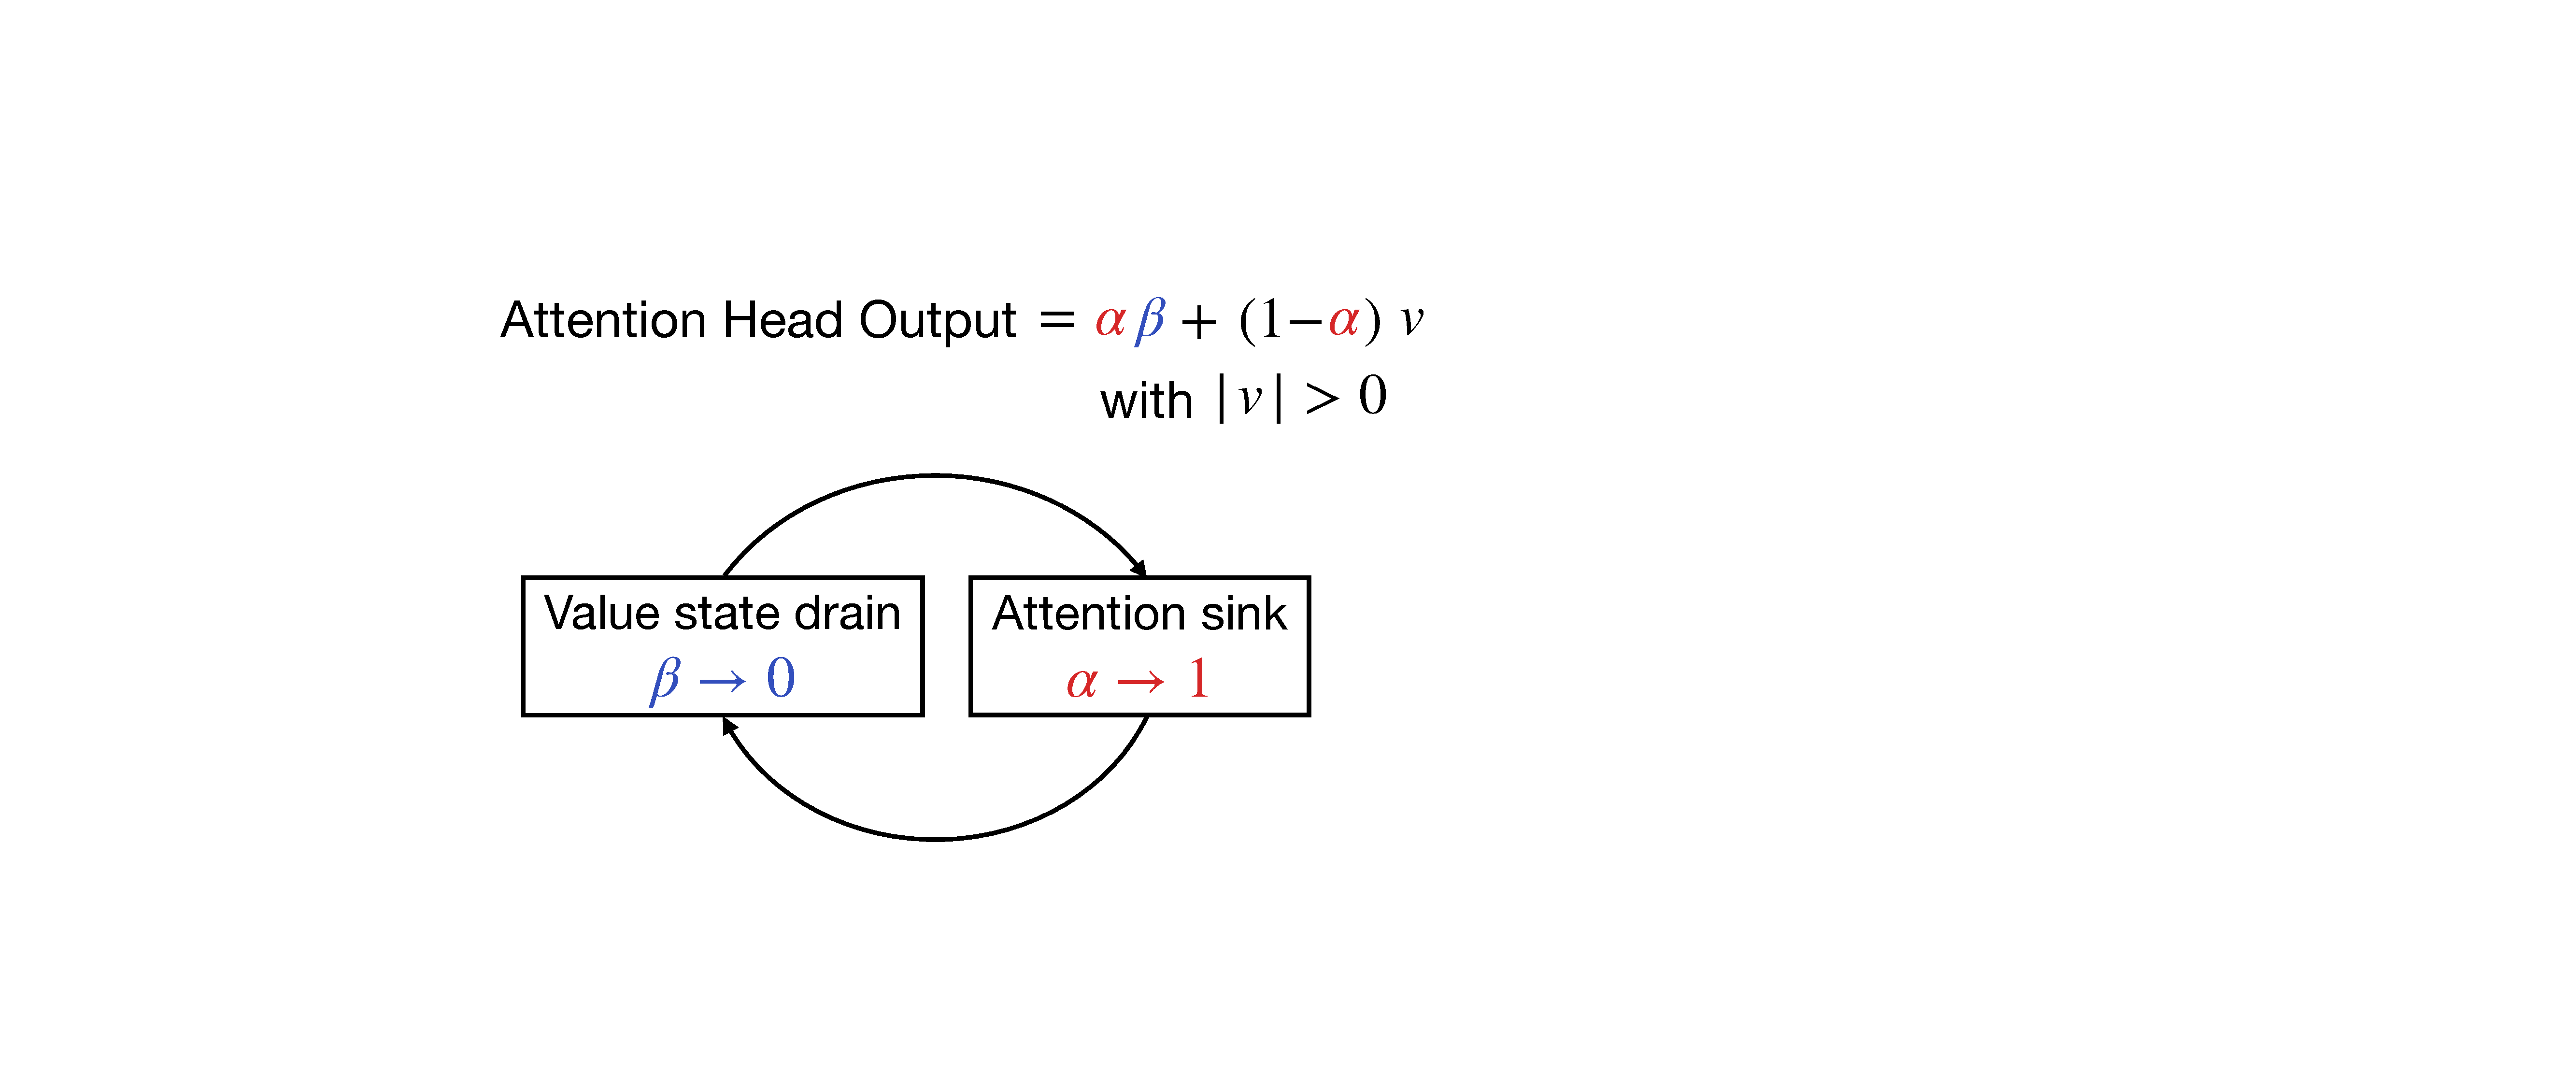
\includegraphics[width=\linewidth]{Figures/illustrations/illlustrations_Part2.pdf}
        \caption{Mutual reinforcement mechanism}
        \label{figure:illustrate-mutual-reinforcement}
    \end{minipage}%
\end{figure}

% \begin{itemize}[leftmargin=2em]
% \setlength\itemsep{0pt}
%     \item[\textup{(a)}] The SoftMax mechanism shifts attention weights towards tokens that exhibit value-state drains, reinforcing these tokens as attention sinks. 
%     \item[\textup{(b)}] Attention sinks on these extreme tokens further suppress their value states, reinforcing their role as value-state drains. 
%     \item[\textup{(c)}] The mutual reinforcement stabilizes when all non-trigger tokens have large, nearly identical attention logits on the extreme token. 
% \end{itemize} 
% Due to the causal mask, the training dynamics favor the \bos~token as the extreme token. 
% \end{claim}

%\sm{This sentence appears here seems weird} \tianyu{I added mutual reinforcement mech}


% \paragraph{combine to the previous paragraph} Although all the $\vecsink=\sink \bm{1}$, $\vecvalue=c\bm{1}-e^{-\sink} \bm{\mass}\circ \bm{\xi}$ are stable phases. Only the phase with $\vecsink\to \infty$ and $\vecvalue\to c \bm{1}$ can match the oracle algorithm with any out of distribution input. When the value $\sink$ is finite, $\vecvalue$ depends on the value $\bm{\mass}\approx \bm{\stable} W$, which strongly depends on the stable distribution $\bm{\stable}$. Therefore, if tested with OOD input that has different stable distribution, it cannot match the oracle algorithm.



\paragraph{Experimental verification of the quantitative prediction.} Revisiting Figure~\ref{fig:dynamics}, which illustrates the dynamics of a single-layer transformer model trained with Adam on the BB task, we observe that $\Delta\text{logit}_{\cdot,\bos}$ exhibits growth rates consistent with Theorem~\ref{thm:main}. In this context, $\Delta\text{logit}_{\cdot,\bos}$  corresponds to $\sink$, as all other attention logits are assumed to be zero under the assumptions of Theorem~\ref{thm:main}. When plotted on a logarithmic scale, the $\Delta\text{logit}_{\cdot,\bos}$ curve grows approximately linearly between 1,000 and 10,000 steps, then accelerates before stabilizing around 100,000 steps.  Meanwhile, the norm of the value state $\|\vall_{\bos}\|_2$ decreases monotonically. The simultaneous increase in attention weights and decrease in value-state norms demonstrate the mutual reinforcement mechanism during the training process. 

To further validate that Theorem~\ref{thm:main} accurately captures the dynamics of the original model, we constructed a simplified model based on Eq.~\eqref{eqn:simplification_TF_1}, \eqref{eqn:simplification_TF_2}, and \eqref{eqn:simplification_TF_3}, and trained the parameters $(\vecsink \in \R^{V}, \vecvalue \in \R^V, \bm{\xi} \in \R^V, \lambda \in \R)$ using Adam. The resulting training curves closely resemble those of the one-layer transformer, also displaying the mutual reinforcement mechanism. A detailed description of the experiment can be found in Appendix~\ref{appsec:train-simple}. 


% P = f(X, V_1, V_2) (ground truth). When P is independent of V_1, V_2, f(X, V_1, V_2) = f(X); Assume p = f(x, 0, 0). Now we fit it with p = f(x, a_1 v_1, a_2 v_2). When v_1, v_2 \neq 0, we need to have a_1, a_2 = 0 to make accurate prediction. 

\paragraph{Generality of the theoretical prediction.} Although Theorem~\ref{thm:main} focuses on a specific BB task with a simplified architecture and loss function, the underlying principles are broadly applicable to more general settings. In particular, we expect that the formation of extreme tokens in LLMs follows a similar mutual reinforcement mechanism. Indeed, Theorem~\ref{thm:main} is essentially based on the following two key assumptions: (1) even with a specific attention head $\attn$ zeroed out, the LLM can still accurately predict the next token, implying that the attention head is better off dormant; and (2) for the attention head $\attn$, value states of previous tokens—except for certain special tokens—remain relevant for specific tasks and therefore do not vanish. Under these assumptions, we anticipate the formation of attention sinks and value-state drains for the attention head $\attn$ and such special tokens. In Section~\ref{sec:llm}, we explore how these phenomena are formed during the training dynamics of LLMs, finding that the empirical results align with the theory. 

% \paragraph{Generality of the theoretical prediction.} Although Theorem~\ref{thm:main} focuses on a specific BB task with a simplified architecture and loss function, the underlying principles are broadly applicable to more general settings. In particular, we anticipate that the formation of extreme tokens in LLMs follows a similar mutual reinforcement mechanism. Specifically, for an attention head $\attn$, we assume that $(\text{LLM}\setminus \attn)(\tok) = \log \bm{\transition}_\tok$, meaning that even with $\attn$ zeroed out, the LLM can still accurately predict the next token. Additionally, we assume $\val(\tok) = \xi_\tok \bm{e}_\tok$, indicating that adding the value state from any previous tokens performs a specific task. Under these assumptions, we expect the same theoretical results to apply. In Section~\ref{sec:llm}, we will explore the formation of extreme-token phenomena along the training dynamics of LLMs, where we find that the empirical results align with the theory. 

\begin{figure}
  \centering
    \begin{minipage}{0.3\textwidth}
      \centering
      \subcaption{\small ReLU attention}
      \label{fig:relu-attn}
      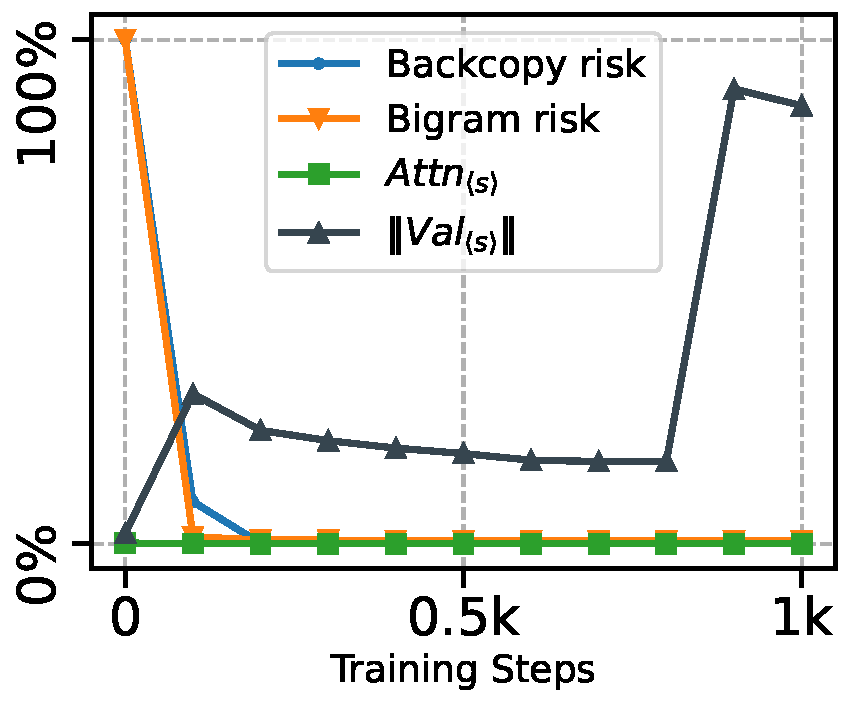
\includegraphics[width=\textwidth]{Figures/BBM/relu_dynamics.pdf}
  \end{minipage}
    \begin{minipage}{0.33\textwidth}
      \centering
      \subcaption{\small Interventions on a 3-layer TF}
      \label{fig:massive-interventions}
      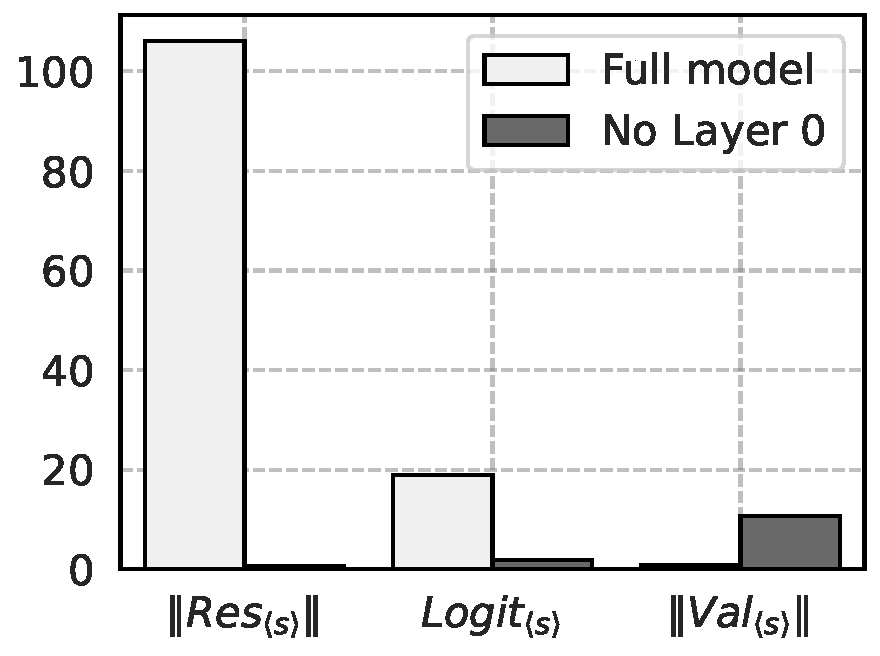
\includegraphics[width=\textwidth]{Figures/BBM/massive_interventions.pdf}
  \end{minipage}
  \begin{minipage}{0.33\textwidth}
      \centering
      \subcaption{\small Eliminating
      residual-state peaks}
      \label{fig:sgd}
      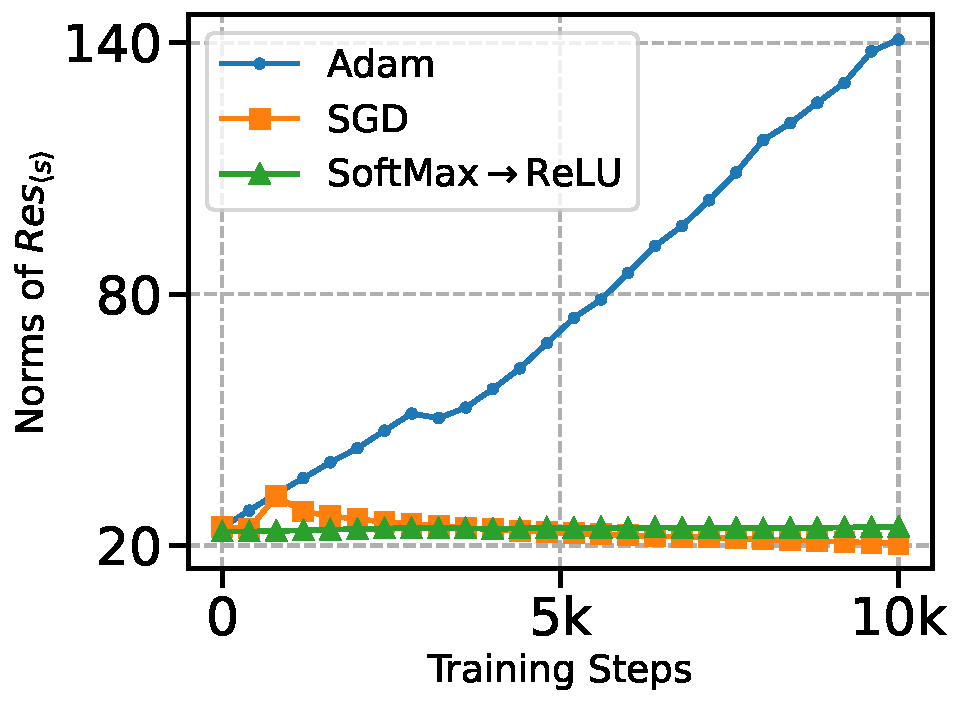
\includegraphics[width=\textwidth]{Figures/BBM/adam_vs_sgd.pdf}
  \end{minipage}
    \caption{\small %\textbf{Experiments on massive norms with multi-layer transformers trained on the Bigram-Backcopy task.} 
    \textit{Left (a)}: The training dynamics of the single-layer ReLU attention transformer on the BB task.
    \textit{Middle (b)}: The intervention results on the \attn+\mlp+\attn+\mlp+\mlp~architecture. The attention sink and value-state peak of the middle $\attn$ layer disappear after zeroing out $\attn+\mlp$ of layer 0. 
    % \tianyu{add which layer for res, logit, and val} \sm{High priority}
    % Figure~\ref{fig:minimal-massive} \sm{no self reference in caption} shows the  $\|\Output(\bos)\|_2$ at layer 0 across different model architectures. 
    \textit{Right (c)}: The evolution of massive norms in a three-layer transformer trained with Adam, SGD, and using a ReLU attention transformer. Notably, only the three-layer model with Softax attention trained using Adam results in the formation of residual-state peaks.}
\end{figure}


\paragraph{Replacing SoftMax by ReLU attention removes attention sinks and value-state drains.} As a consequence of our theory, we predict that training using ReLU attention in place of SoftMax attention will prevent the mutual reinforcement mechanism. Without SoftMax, the training dynamics no longer push the attention weights toward the \bos~token, which remains zero throughout training. In the absence of attention sinks, the dynamics no longer push down the value state norm, and the mutual reinforcement mechanism breaks. Figure~\ref{fig:relu-attn} presents the training dynamics on the BB task using ReLU instead of SoftMax attention, showing that both the Bigram and Backcopy risk converge to the Bayes risk after 200 training steps, but the attention logits of \bos~do not increase, and the value state does not shrink, confirming our prediction. 


\subsection{The emergence of residual-state peaks}
\label{sec:res-peak}
In this section, we experimentally investigate the residual-state peaks phenomenon. We observe that no residual-state peaks occur in the single-layer transformer trained on the BB task. To explore this further, we train slightly deeper transformers on the BB task and track the residual state norm after layer $0$. We observe that two-layer models do not exhibit residual-state peaks, while models with three or more layers do.
% track the residual state norms of the \bos~token at the output of layer 0.
Additional experimental results are provided in Appendix~\ref{appsec:mini-res-peak} and \ref{appsec:three-layer-tf}. 
% \paragraph{The residual-state peaks require a three-layer structure.} \tianyu{change the claim to that layer 0 has residual state peak, but layer 1 does not} A three-layer transformer is enough to produce residual-state peaks. 
% In Figure~\ref{fig:minimal-massive},  
% If we allow the skipping of some \mlp~or \attn~layers, the ``\attn+\mlp+\attn+\mlp+\mlp'' combination becomes the simplest model that produces residual-state peaks (Figure~\ref{appfigure:massive_minimal}). Circuit analysis reveals that LLMs typically add a large vector in the first layer and cancel it in the last layer, coinciding with the findings in \cite{sun2024massive}. \sm{I added this part. Did they already propose this?} We hypothesize that the add-then-cancel mechanism is essential for residual-state peaks and requires at least three layers.

% \paragraph{Residual state peak reinforces attention sinks and value-state drains in trained models.} Figure~\ref{fig:massive-interventions} presents the intervention results on the ```\attn+\mlp+\attn+\mlp+\mlp'' model. We recenter the $\|\res_{\bos}\|_2$ by subtracting the average norm of other tokens from the \bos~token norm. The $\text{logit}_{\cdot,\bos}$ and $\|\val_{\bos}\|$ are computed in layer $1$ following the same ways as in Figure~\ref{fig:dynamics}. When layer 0 is zeroed out, the residual norm returns to normal, attention logits decrease, and the value state norm rises. It verifies that the residual-state peak contributes to the attention sink and value-state drain phenomenon in the trained transformer.

% \paragraph{Massive residual state at layer 0 output induces attention sinks and value-state drains in the middle layer.} To investigate the influence of residual-state peak at layer 0 output on attention sinks and value-state drains in the middle layer, we implement intervention experiments in the ``\attn+\mlp+\attn+\mlp+\mlp'' model. We compute the difference of $\|\res_\bos\|$ and $\text{Mean}_\tok[\|\res_\tok\|]$ at layer 0 output, and compute $\text{logit}_{\cdot,\bos}$ and $\|\val_{\bos}\|$ in the middle layer following the same ways as in Figure~\ref{fig:dynamics}. When layer $0$ (the first ``\attn+\mlp'' block) is zeroed out, the residual state norm becomes non-massive, attention logits and the value state norm returns to normal. It verifies that the residual-state peak contributes to the attention sink and value-state-drain phenomenon in the middle layer of trained transformers. 

% \paragraph{Residual-state peak is induced by the output of layer 0 in transformers with at least three layers.} We observe that two-layer models do not exhibit residual-state peaks, while models with three or more layers do.
% Intervention experiments confirm that the residual-state peaks are induced by the layer $0$, with other layers having negligible effect on the residual state norm. 

% \paragraph{Residual-state norm become massive in layer 0 output and return to normal in layer 1 output.} 

\paragraph{Massive residual state at layer 0 output induces attention sinks and value-state drains in the middle layer.} To investigate the relationship between massive residual states and attention sinks, we train on the BB task using the ``\attn+\mlp+\attn+\mlp+\mlp'' model, which is the minimal structure that shows the massive residual states phenomena. We perform intervention by analyzing how the model's behavior changes after zeroing out layer 0 (the first ``\attn+\mlp'' block). Before and after zeroing, we compute the difference in $\|\res_\bos\|$ and $\text{Mean}_\tok[\|\res_\tok\|]$ at the layer 0 output, and compute $\text{logit}_{\cdot,\bos}$ and $\|\val_{\bos}\|$ in the middle layer. After zeroing out, the residual state norm becomes non-massive, and attention logits and the value state norm return to a normal level. This confirms that the residual-state peak contributes to the attention sink and value-state-drain phenomena in the middle layer of pre-trained transformers. 

%\sm{We didn't introduce why we perform intervention on this model}


% \paragraph{I plan to put the theory for residual-state peaks part in the appendix} To include the 
% To model the dynamics of massive norms, we assume that $\cos(\query_i, \key_0)=1$ for any $i$. The output of the lower layer adds $m \key_0/\ltwo{\key_0}$ on the residual stream of the \bos~token and get $\bh_0+m\key_0$. Assume that $\ltwo{\bh}=1$ and $\cos(\bh, \key_0) = c$. As a result,  

\paragraph{Linear growth of residual-state norm with Adam training.} Figure~\ref{fig:sgd} shows the residual-state norms of the \bos~token at the layer 0 output of three-layer transformers during pre-training on the BB task. The results indicate that training the transformer with Adam leads to a linear increase in residual state norms.

\paragraph{Switching from Adam to SGD and switching from SoftMax to ReLU attention eliminates the residual-state peaks.} Figure~\ref{fig:sgd} also illustrates the dynamics of residual-state norms in other training setups. When switching the training algorithm from Adam to SGD, attention sinks remain, but residual-state peaks disappear. Similarly, switching to ReLU attention, which lacks the mutual reinforcement mechanism, also eliminates residual-state peaks. These findings highlight the dependence of residual-state peaks on SoftMax attention and the Adam optimization algorithm. We propose a potential explanation of this phenomenon in Appendix~\ref{appsec:theory-for-res}. 


% \begin{claim}[Potential mechanism for the formation of residual-state peaks]\label{claim:res-peak}
% In the training dynamic of a multi-layer transformer, if the mutual reinforcement mechanism (cf.\ Claim~\ref{claim:mutual-reinforcement}) occurs in upper layers:
% \begin{enumerate}
%     \item The gradients of $\res_\bos$ have the same direction (aligning with the null space of value matrices in upper layers and the $\key_\bos$) along the training dynamics.
%     \item The layer norms cause the fast decay of the magnitude of the gradients.
%     \item Adam induces diminishing gradients to be constant updates, leading to the linear growth for the norm of the residual state of the extreme token.
% \end{enumerate}
% \end{claim}

% Therefore, we hypothesize that the \activedormant~strengthens their formation. Specifically, when the training dynamics push the attention logits on the \bos~token, it also pushes up the norm of $\vall_{\bos}$ and $\mlp_{\bos}$ in layer 0. Due to the layer norm, their gradients shrink quickly, but Adam makes small gradients constant updates, leading to a linear increase in residual norms.


% \begin{itemize}
%     \item The attention sinks and value-state drains are external manifestations of the active-dormant mechanism in LLMs.
%     \item The attention heads go through the attention-increasing and value-state-shrinking phases. They converge to the stable phase with identical attention logits on the \bos~token.
%     \item The residual-state peaks reinforce attention sinks and value-state drains. Both the lower layer attentions and MLPs contribute to the residual-state peaks.
%     \item The residual states go through linear increasing phase in the pre-training.
% \end{itemize}


% \subsection{Verify the predictions from the theory}



